\section{\framework{} Methodology}
\label{sec:methodology}

We now provide the methodology to achieve the goal of deceiving user data fed to the apps without rooting the device or altering the source of the apps.

\subsection{Background on Hooking}
In Android, users cannot typically modify app or OS behavior, but \textit{hooking} provides a practical method to alter execution flow by injecting new instructions.

Hooking can be static or dynamic. Static hooking modifies bytecode or injects shared libraries pre-execution, making permanent changes detectable via digital signature verification. Dynamic hooking alters volatile memory at runtime, enabling temporary modifications based on execution context. Android's Dalvik VM uses Dynamic Linkers' "virtual method table" for method calls, allowing \textit{Call Diversion} to inject hooks into the lookup table.

The \texttt{boot.oat} and \texttt{boot.art} files optimize boot speed by storing frequently used class source code and a pre-initialized heap. The target class's heap resides in \texttt{boot.art}, while \texttt{app.dex} and \texttt{libart.so} store the app's Dalvik Executable code and shared libraries. When the app calls a target method, the system retrieves the method's address from virtual tables in the heap and executes it.

Figure \ref{fig:vrtulMemMthdCall} illustrates dynamic hooking in Android using \texttt{getLatitude()}. Figure \ref{fig:vrtulMemMthdCall_woFr} shows the standard method call process, where app's virtual memory includes heap space and files loaded by \textit{Zygote}. Initialized at OS boot, it preloads Java shared libraries to speed up app launches. When an app calls a method, the system retrieves its address from virtual tables in the heap and executes it.

\begin{figure}[t]
    \centering
    \begin{subfigure}{0.48\linewidth}
        \vspace{7mm}
        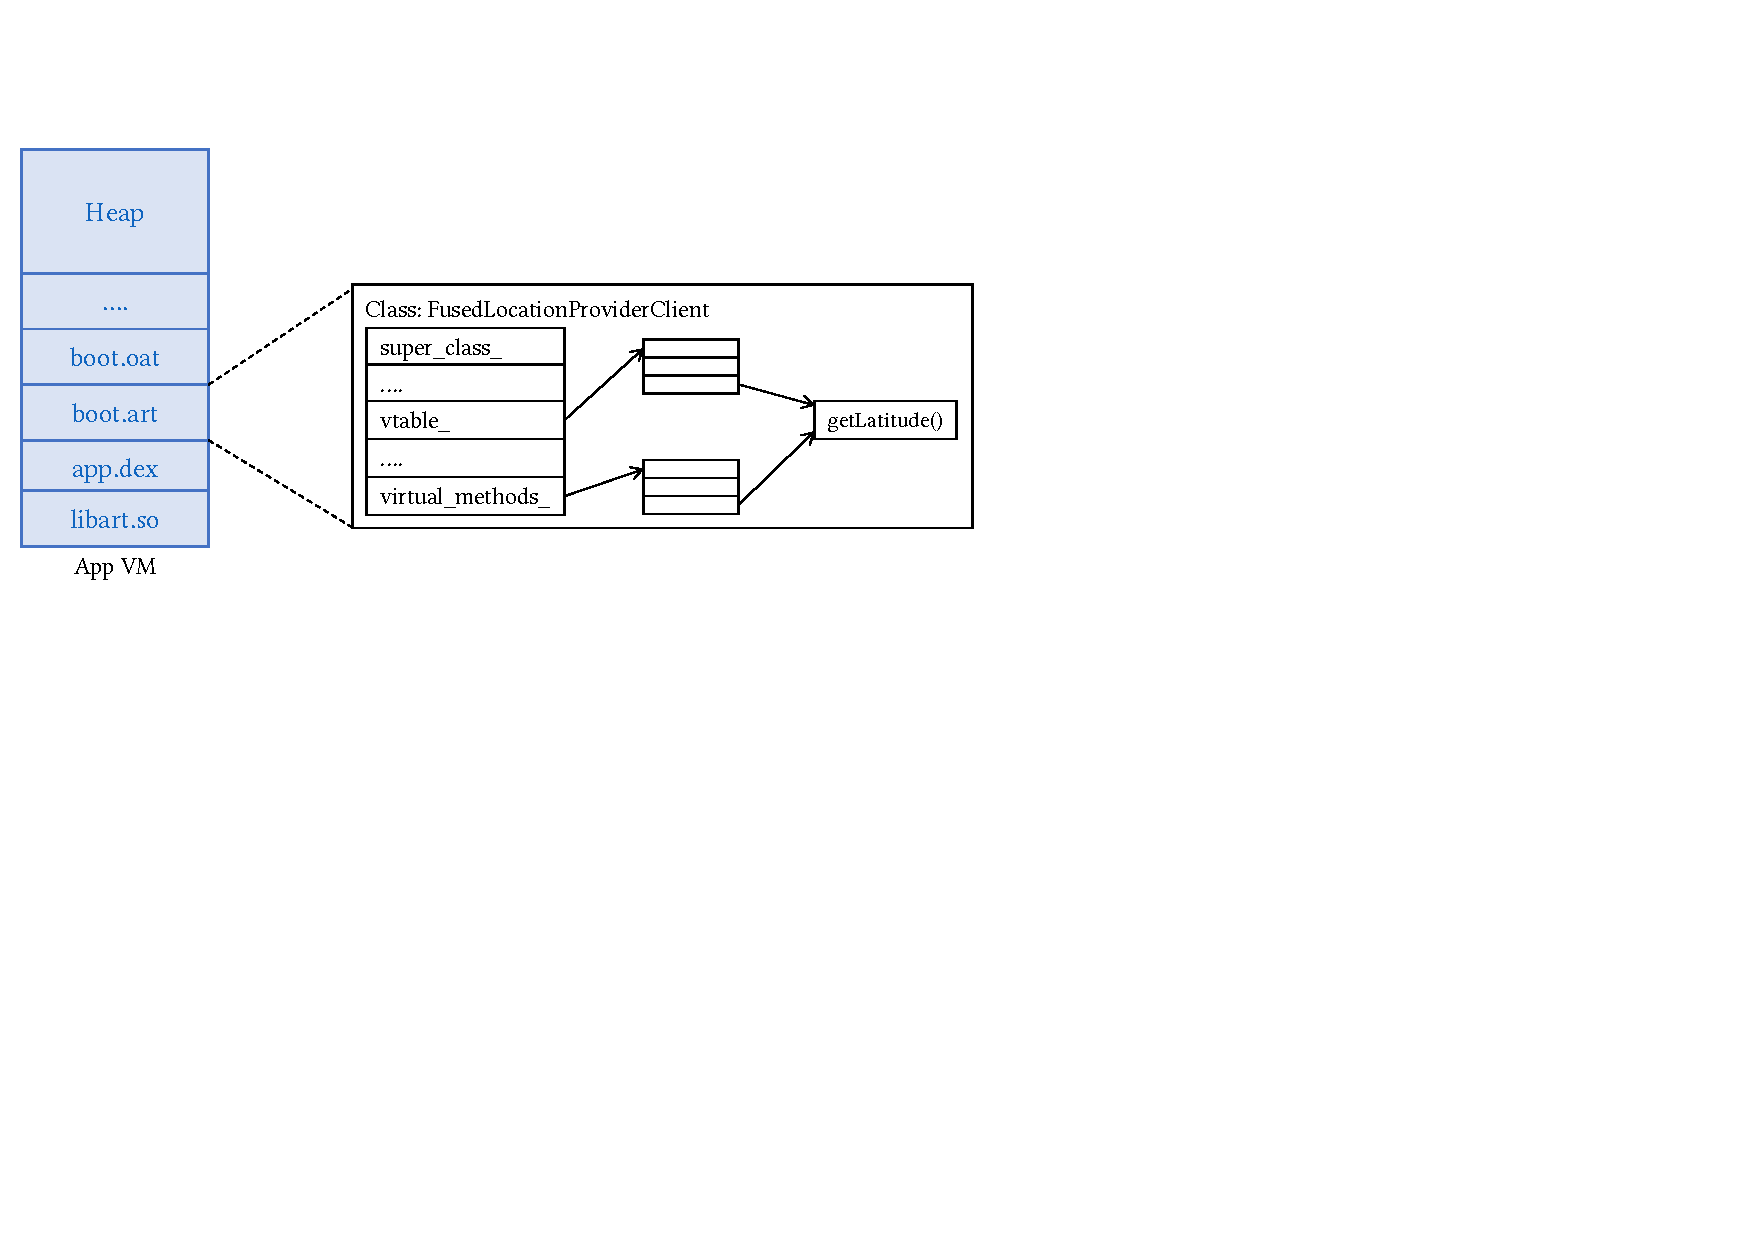
\includegraphics[width=\linewidth]{Figures/Background/virtual_memory_without_deceiver.pdf}
        \caption{Original method call.}
        \label{fig:vrtulMemMthdCall_woFr}
    \end{subfigure}
    \begin{subfigure}{0.48\linewidth}
        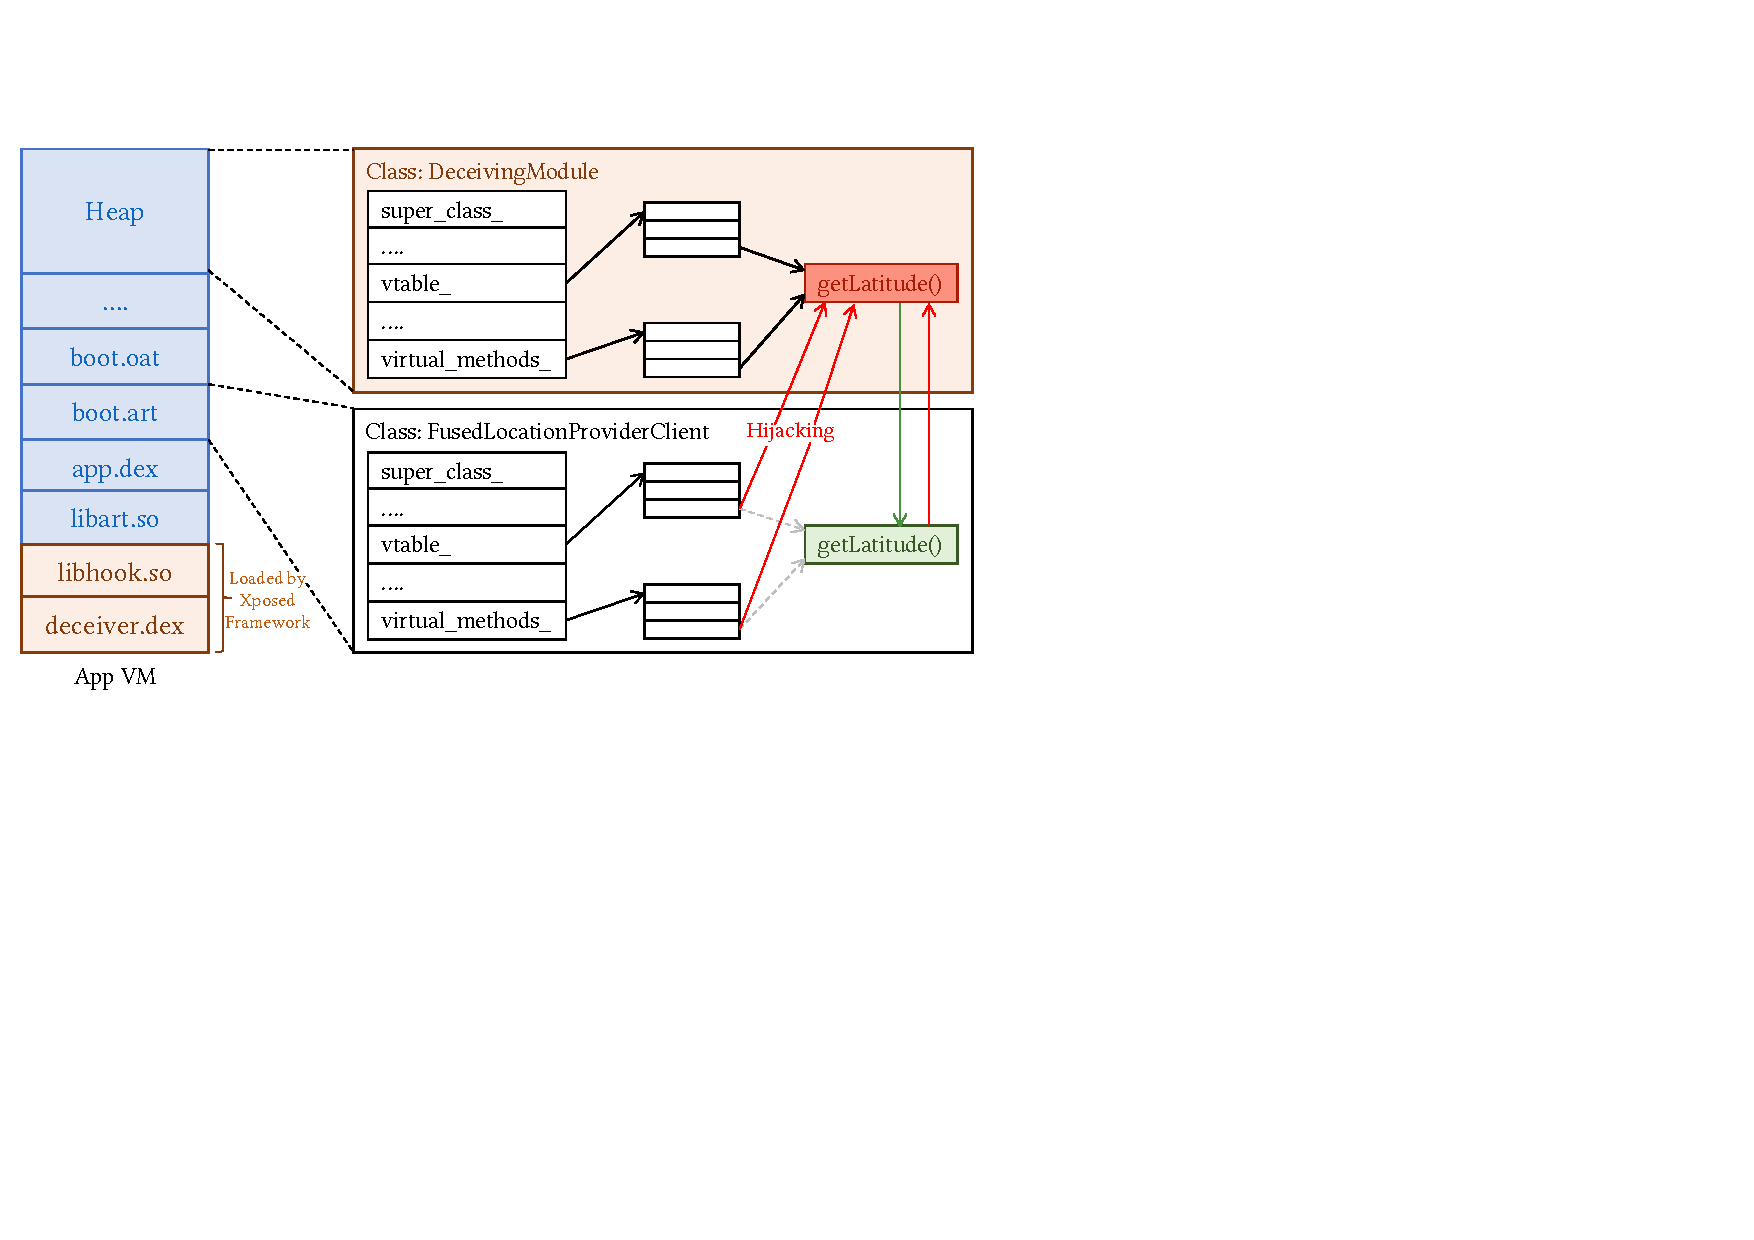
\includegraphics[width=\linewidth]{Figures/Background/virtual_memory_with_deceiver.pdf}
        \caption{Method call with \framework{}.}
        \label{fig:vrtulMemMthdCall_wFr}
    \end{subfigure}
    \caption{Example illustrating how the Xposed module class method hijacks the original method call.}
    \label{fig:vrtulMemMthdCall}
\end{figure}

Figure \ref{fig:vrtulMemMthdCall_wFr} illustrates the hooking process, where the hooking module loads \texttt{libhook.so} into the app's memory and injects hooks from \texttt{hook.dex} as Dalvik Executables. \texttt{libhook.so} modifies the heap by replacing virtual table entries of target classes with hooking method addresses, redirecting method calls to hooking methods, which invoke the original method at the end.


\subsection{Hooking on Non-Rooted Device}

App hooking is the most effective way to spoof user data, but non-rooted devices lack system process hooking, as root access to \textit{Zygote} is not present.

We achieve this via \textit{adb} (Android Debug Bridge), which grants privileged system API access while connected. To bypass this, we use \textit{Shizuku}, which runs a dedicated process with shell-level permissions, acting as a proxy between apps and the OS—sufficient for hooking. With Shizuku, we utilize \textit{LSPatch}, an Xposed framework for non-rooted devices, to inject hooks into app processes. This enables custom behavior via the Xposed module while ensuring target apps function properly. Both Shizuku and LSPatch are open-source, granting root privileges only to selected modules and apps, preserving security.

\subsection{Spoofing User Data with Hooking}

Listing \ref{lst:clipboardDeceiver} illustrates how clipboard data can be spoofed using hooking. Apps typically retrieve clipboard content via \texttt{ClipboardManager.getPrimaryClip()}, but modifying its output requires hooking multiple methods. A more efficient alternative is hooking \texttt{ClipData.CREATOR.createFromParcel()}, as it is the final method invoked to return clipboard data. This is achieved using Xposed's \texttt{handleLoadPackage()} (Line~3).

With this approach, clipboard data can be blocked or modified before reaching target apps. The before hook (Lines 7-14) blocks clipboard access by retrieving the user's preference via \textit{ContentProvider} (Lines 9-13). If blocking is enabled (Line 15), the function returns a null object, preventing the original method from executing.

Similarly, the after hook (Lines 16-25) replaces clipboard content with user-defined spoofed data. The spoofed text is retrieved from \textit{ContentProvider} (Lines 19-22) and used to initialize a new \texttt{ClipData} object (Line 24).

\framework{} also offers various permission-spoofing policies. For example, it blurs images when an app accesses the camera in the background, detected via \texttt{ActivityManager}, by manipulating pixel data. Another policy injects noise into the audio feed if an app requests microphone access without a valid reason.

\subsection{\framework{} and its Robustness}
This section outlines \framework{}'s approach to spoofing user data and evaluates its effectiveness in real-world applications, demonstrating its robustness.

\mysubsubsection{Robust Mechanism} \framework{} employs dynamic hooking to modify user data in volatile memory without altering disk storage, making it undetectable via APK signatures or \textit{Play Integrity} API. Instead of revoking permissions, it contextually spoofs data, ensuring app stability and a crash-proof user experience.

\mysubsubsection{Real-World Evaluation} \framework{} was tested on 50 Google Play Store apps and 20 pre-installed Android apps. All permissions were granted, and each app was manually used for 20 minutes on a \textit{Samsung Galaxy M21} (2.3 GHz octa-core processor, 4 GB RAM, Android 12). Results were verified through visual confirmation of spoofed data and \framework{}'s logs.

Figure \ref{fig:intro_heatmap} presents \framework{}'s performance, where dark green, light green, orange, and red represent permissions that were successfully deceived, not requested, not used, or not deceivable, respectively. Out of 678 requested permis-

\begin{lstlisting}[caption={Kotlin code to deceive Clipboard permission data with the data defined by user in \textit{Deceit} policies.},label={lst:clipboardDeceiver},language=Kotlin,float=*]
class SpoofingModule: IXposedHookLoadPackage {
    companion object {
        fun getClass(clsName: String): Class<*> = Class.forName(clsName, false, lpparam.classLoader)    
    }
    
    @Throws(Throwable::class)
    override fun handleLoadPackage(lpparam: XC_LoadPackage.LoadPackageParam) {
        hookAllMethods(getClass(ClipData.CREATOR.javaClass.name), "createFromParcel", XC_MethodHook() {
            @Throws(Throwable::class)
            override fun beforeHookedMethod(param: MethodHookParam) {
                val uri = Uri.parse("content://com.xposedModule.provider/deceitSettings")
                val cursor = context.contentResolver.query(uri, null, null, null, null) ?: return
                val blockClipboard = cursor.getInt(cursor.getColumnIndex("blockClipboard")
                cursor.close()
                if(blockClipboard) param.result = null
            }

            @Throws(Throwable::class)
            override fun afterHookedMethod(param: MethodHookParam) {
                param.result ?: return
                val uri = Uri.parse("content://com.xposedModule.provider/deceits")
                val cursor = context.contentResolver.query(uri, null, null, null, null) ?: return
                val clipboardLabel = cursor.getString(getColumnIndex("clipboardLabel")) ?: "dummyLabel"
                val clipboardText = cursor.getString(getColumnIndex("clipboardText")) ?: "dummyText"  
                cursor.close()
                param.result = ClipData.newPlainText(clipboardLabel, clipboardText)
            }       
        })   
    }
}
\end{lstlisting}

\begin{figure}
    \centering
    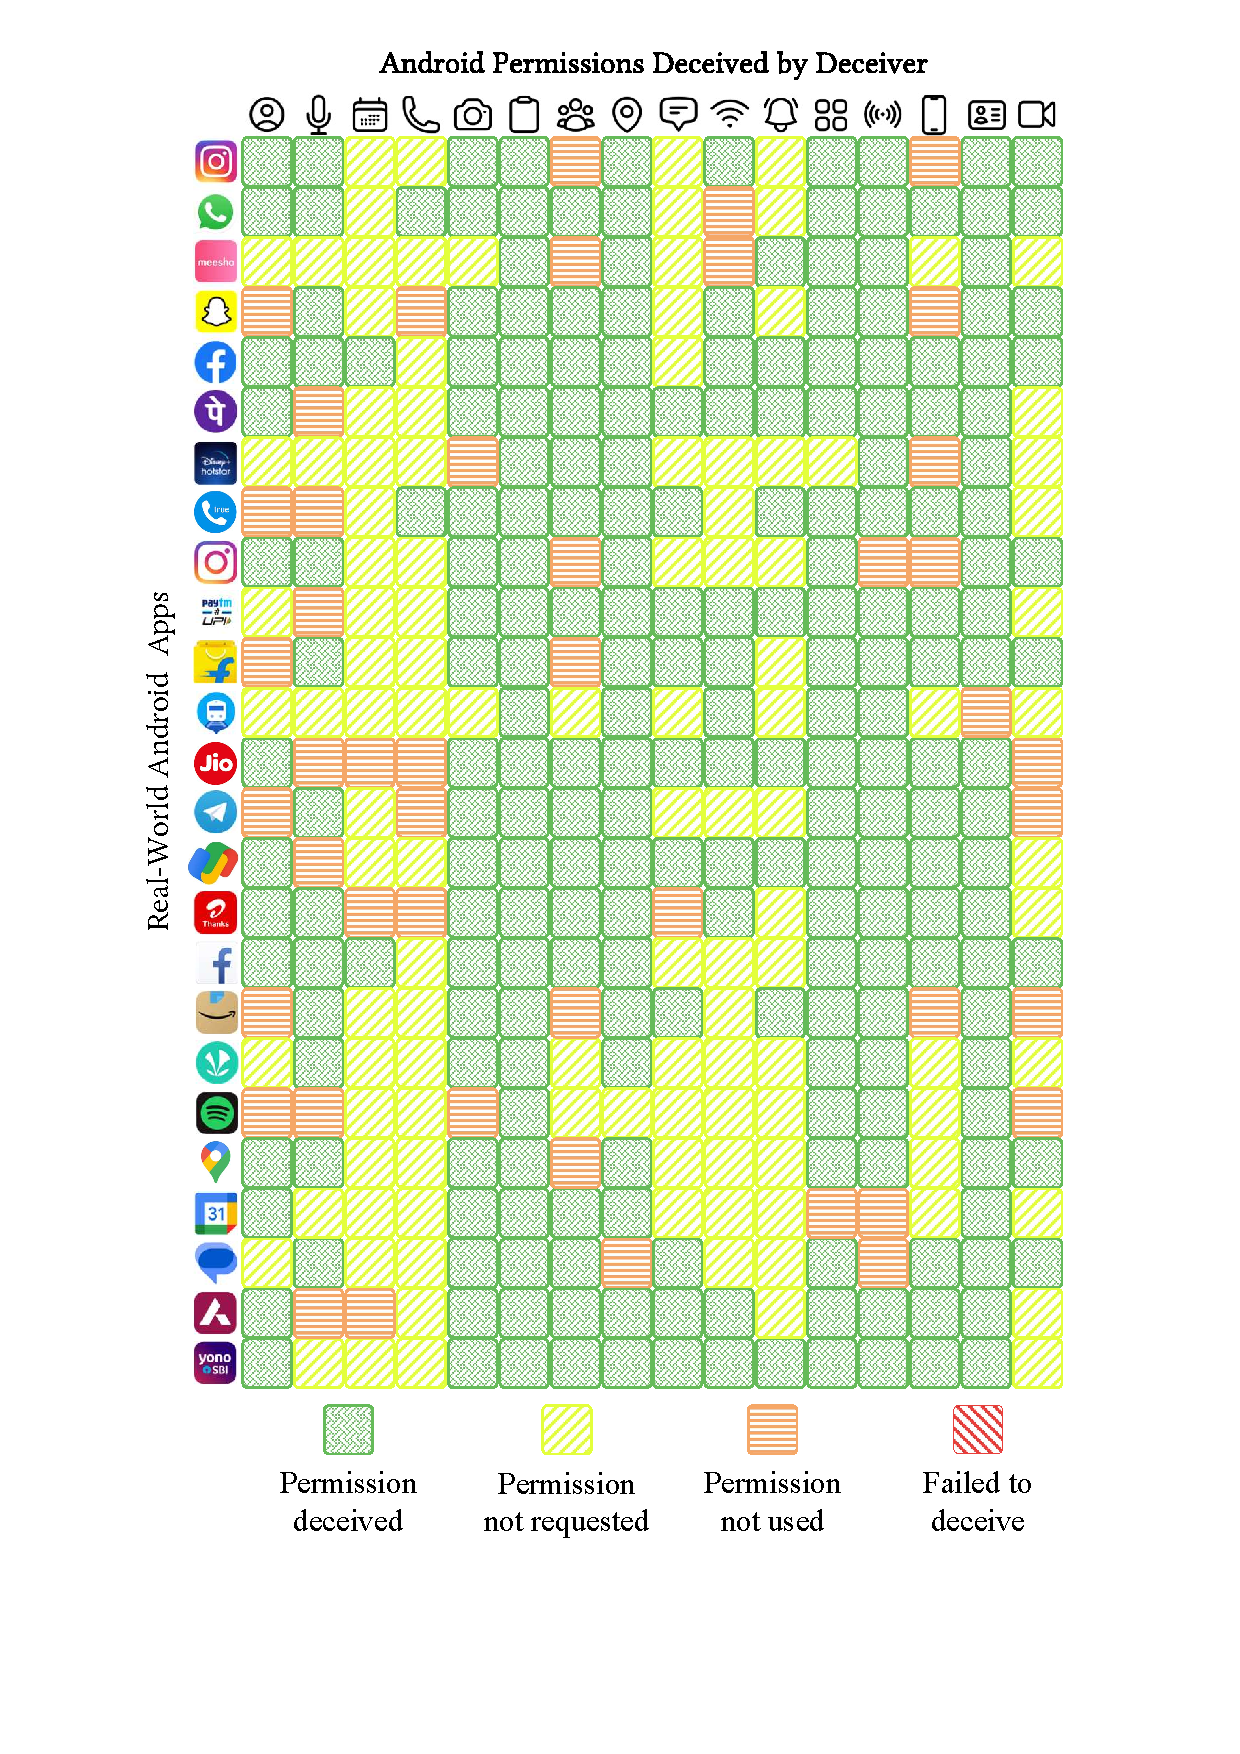
\includegraphics[width=0.6\linewidth]{Figures/Introduction/heatmap.pdf}
    \caption{Heatmap illustrating status of user data deceived for various popular apps by \framework{}.}
    \label{fig:intro_heatmap}
    \vspace{-20pt}
\end{figure}

\noindent sions, \framework{} successfully spoofed 78.32\%, while 21.68\% could not be verified as they were not explicitly utilized. The results confirm \framework{}'s robustness, as no app crashed, and all functioned as expected.

% \mysubsubsection{Hooking Hidden APIs} Certain permissions, like those involving sensors, rely on \textit{Android Non-SDK Interfaces} (\textit{Hidden APIs}) such as \texttt{InputSensorInfo}, which are restricted for \textit{JNI} and \textit{Java Reflections}. \framework{} circumvents these restrictions using \textit{LSPlant} to instantiate classes with spoofed data. Notably, 23.16\% of successful spoofing was achieved through Hidden API hooking, demonstrating \framework{}'s ability to bypass Android's access limitations.

% \mysubsubsection{Secure and Isolated Operation} \framework{} requires only the \textit{Query All Packages} permission, a non-runtime (normal) permission, to enhance its privacy protection features. It operates entirely offline, ensuring no external connections and maintaining a secure, trustworthy environment.
